\section{Use Existing Point of Sale Infrastructure}
\label{sec:goals-infrastructure}

While constructing new and better protocols is an effective way to defend against attacks,
	a requirement to modify or update widely established infrastructure imposes a significant barrier to the adoption of this new protocol.
For example, in order to implement the Secure CC Protocol described previously in Chapter \ref{cha:secure}, every point of sale must be modified or replaced.
In order to sidestep this barrier, we consider the protocol in use today (the Insecure CC Protocol in Chapter \ref{cha:insecure}) from the perspective of a point of sale.

A point of sale may do rudimentary checks on the structure of the Card Information messages that it receives,
	but it relies on the bank in order to validate the data in these messages.
The Insecure CC Protocol, from the perspective of the point of sale, is illustrated in Figure \ref{fig:interface_pos} and operates as follows:

\begin{enumerate}
\item The point of sale issues a Solicitation message over the NFC channel.
	This message contains no payload of interest.
\item The point of sale receives a Card Information message over the NFC channel.
	This message consists of the following fields:
	\begin{itemize}
	\item a 16-digit card number
	\item a 4-digit expiration date
	\item an 8-digit iCVV
	\end{itemize}
	In practice, this is an opaque\footnote{
        There are some constraints on this value.
        For example, an expiration date of ``8321'' does not need to be verified by a bank to be declared invalid.
        Similarly, there are constraints on credit card numbers as well.
        These have little effect on our approach, so we ignore them for simplicity.
    }
    28-digit numeric value (16 + 4 + 8).
    This data is accompanied by the bank name.
\item After receiving the Card Information message,
	the point of sale issues a Charge Request message to the bank specified by the bank name field in the Card Information message.
	The Charge Request message consists of the card's credit card number, expiration date, iCVV, and the price to charge.
	In practice, this repeats the same 28-digit numeric value received in the Card Information message, accompanied by the price to charge.
\item Later, the point of sale receives an Approval message in response to the Charge Request message.
	The Approval message consists of the bank's decision on whether to accept the charge, as described in Section \ref{sec:insecure-design}.
\end{enumerate}

\begin{figure}[h!]
  \caption{Insecure CC Protocol, Point of Sale Behavior}
  \centering
    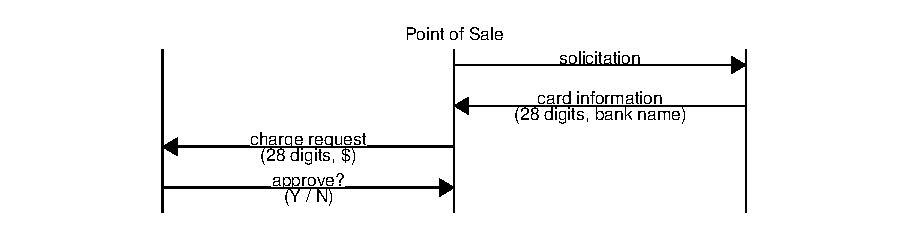
\includegraphics{img/interface_pos.eps}
  \label{fig:interface_pos}
\end{figure}

A key observation of the point of sale's behavior is that it consists of relaying data
	specified by the card to a destination \emph{also specified by the card}.
While the point of sale may interpret the 28-digit data content of the Card Information message as consisting of three fields describing a credit card,
	the customer may instead use these fields to encode an arbitrary 28-digit message, provided that the recipient of the Charge Request message decodes it accordingly.

We leverage this observation in the construction of the Unlinkable Wallet Protocol to conform to existing point of sale behavior,
	by using this 28-digit message as a carrier for the data we wish to transmit.
In so doing, we ensure that the point of sale in the Unlinkable Wallet Protocol remains identical to its counterpart in the Insecure CC Protocol.
